\documentclass{article}

\usepackage{tikz-feynman}

\begin{document}

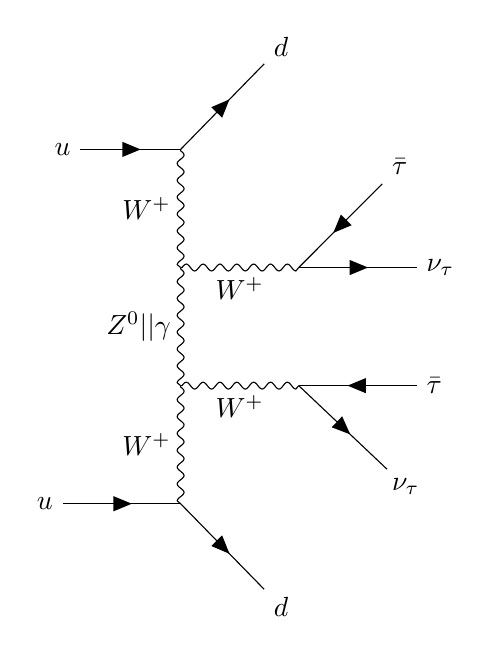
\begin{tikzpicture}
\begin{feynman}
\vertex (a) {\(u\)};
\vertex [right=of a](b);
\vertex [above right=of b](c){\(d\)};
\vertex [below=of b] (d);
\vertex [below=of d] (e);
\vertex [below=of e] (f);
\vertex [left=of f] (g) {\(u\)};
\vertex [below right=of f] (h) {\(d\)};
\vertex [right=of d] (i);
\vertex [above right=of i] (l){\(\bar{\tau}\)};
\vertex [right=of i] (m){\(\nu_{\tau}\)};
\vertex [right=of e] (o);
\vertex [right=of o] (p){\(\bar{\tau}\)};
\vertex [below right=of o] (q){\(\nu_{\tau}\)};


\diagram* {
	(a) -- [fermion] (b) -- [fermion] (c),
	(b) -- [boson, edge label'=\(W^{+}\)] (d) -- [boson, edge label'=\(Z^{0} ||  \gamma\)] (e) -- [boson, edge label'=\(W^{+}\)] (f);
	(g) -- [fermion] (f) -- [fermion] (h);
	(d) -- [boson, edge label'=\(W^{+}\)] (i);
	(l) -- [fermion] (i) -- [fermion] (m);
	(e) -- [boson, edge label'=\(W^{+}\)] (o);
	(p) -- [fermion] (o) -- [fermion] (q);
};
\end{feynman}
\end{tikzpicture}

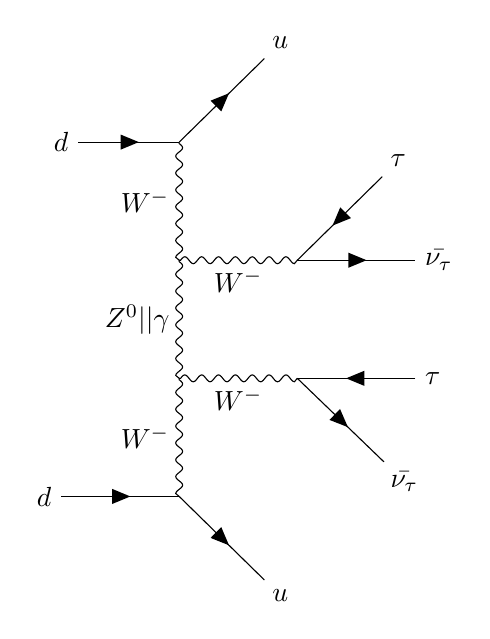
\begin{tikzpicture}
\begin{feynman}
\vertex (a) {\(d\)};
\vertex [right=of a](b);
\vertex [above right=of b](c){\(u\)};
\vertex [below=of b] (d);
\vertex [below=of d] (e);
\vertex [below=of e] (f);
\vertex [left=of f] (g) {\(d\)};
\vertex [below right=of f] (h) {\(u\)};
\vertex [right=of d] (i);
\vertex [above right=of i] (l){\(\tau\)};
\vertex [right=of i] (m){\(\bar{\nu_{\tau}}\)};
\vertex [right=of e] (o);
\vertex [right=of o] (p){\(\tau\)};
\vertex [below right=of o] (q){\(\bar{\nu_{\tau}}\)};


\diagram* {
	(a) -- [fermion] (b) -- [fermion] (c),
	(b) -- [boson, edge label'=\(W^{-}\)] (d) -- [boson, edge label'=\(Z^{0} ||  \gamma\)] (e) -- [boson, edge label'=\(W^{-}\)] (f);
	(g) -- [fermion] (f) -- [fermion] (h);
	(d) -- [boson, edge label'=\(W^{-}\)] (i);
	(l) -- [fermion] (i) -- [fermion] (m);
	(e) -- [boson, edge label'=\(W^{-}\)] (o);
	(p) -- [fermion] (o) -- [fermion] (q);
};
\end{feynman}
\end{tikzpicture}

\end{document}
